\section{Interfaz gráfica}\label{sec:interfaz}

\subsection{Arquitectura de la app}
La interfaz se construyó en \textbf{Streamlit} (web local con \texttt{streamlit run}), confirmada como aceptable por el docente. Se organizó en cuatro pestañas con \texttt{st.tabs}, todas operativas en macOS y Windows. El código vive en \texttt{app/streamlit\_app.py}.

\subsection{Contrato de preprocesamiento compartido}
La regla metodológica más importante del Bloque G es que \textbf{la interfaz nunca recodifica a mano}. Toda transformación de entrada pasa por la función compartida \texttt{preparar\_entrada(dict) -> np.array} en \texttt{src/preprocessing.py}, importada tanto por el notebook de preprocesamiento como por la app. Misma función = imposible divergir. La función consume \texttt{models/feature\_list.json}, \texttt{models/scaler.pkl} y \texttt{models/encoders.pkl}, lo que garantiza que el vector de entrada tenga exactamente las 72 columnas en el orden correcto.

\subsection{Pestañas}
\subsubsection{Pestaña 1: Predicción de severidad}
Formulario con \emph{selectbox} para departamento y modalidad, \emph{date\_input} para fecha, \emph{slider} 0--23 para hora, \emph{text\_input} para el código de vía y \emph{number\_input} $\geq 0$ para kilómetro. Al pulsar ``Analizar riesgo'' se muestra:
\begin{itemize}
  \item Un medidor tipo \emph{gauge} (Plotly) con la probabilidad de accidente mortal (0--100\,\%) y zonas de color según el umbral de \texttt{threshold.json} (verde bajo, ámbar medio, rojo alto).
  \item Una etiqueta grande MORTAL / NO MORTAL según el umbral.
  \item Una explicación del caso basada en los top-5 factores globales del modelo y los valores ingresados. Si SHAP local responde en menos de 2 segundos, se añade como complemento; si demora o rompe la demo, no se fuerza y queda para el informe.
  \item Una nota de alcance al pie: ``Estimación de factores de riesgo con fines académicos; no es un predictor determinista.''
\end{itemize}
La salida natural de un modelo de clasificación es un medidor de probabilidad (\emph{gauge}), no un gráfico de líneas; este último se usa para pronóstico de series continuas en el tiempo, que no es el caso.

\subsubsection{Pestaña 2: Análisis exploratorio}
Replica con Plotly interactivo los hallazgos del Bloque C: tasa de mortalidad por modalidad, accidentes por hora del día, tasa de mortalidad por hora, serie temporal mensual de accidentes y distribución del target. Cada gráfico con 1--2 líneas de lectura.

\subsubsection{Pestaña 3: Riesgo por departamento}
Ranking interactivo por departamento (barras y tabla ordenable) con número de accidentes y tasa de mortalidad. El mapa coroplético con GeoJSON de departamentos se consideró como mejora opcional; el ranking por barras es prioridad obligatoria y funciona sin dependencia externa.

\subsubsection{Pestaña 4: Sobre el modelo}
Arquitectura del modelo (\texttt{model.summary()}), tabla comparativa contra las líneas base, matriz de confusión, curvas ROC y Precision-Recall, ficha del dataset y declaración de la regla anti-fuga. Cierra con créditos del equipo, curso y universidad.

\subsection{Pruebas funcionales}
El checklist del Bloque G (\texttt{tab09\_gui\_checklist.csv}) verificó:
\begin{itemize}
  \item Las cuatro pestañas cargan sin error.
  \item El caso típico responde en menos de 2 segundos.
  \item Cambiar solo la modalidad de baja letalidad a ATROPELLO sube la probabilidad de modo coherente con el EDA (demo\_02: 0.30 $\rightarrow$ 0.80).
  \item La hora nocturna vs.\ diurna produce cambios razonables (demo\_03: 0.30 $\rightarrow$ 0.33).
  \item Un código de vía no visto no rompe la app y mapea \texttt{via\_freq = 0} (demo\_04: 0.30).
  \item La pestaña departamental funciona como barras/ranking.
\end{itemize}

\subsection{Capturas}
\begin{figure}[H]
  \centering
  \begin{minipage}{0.49\textwidth}\centering
    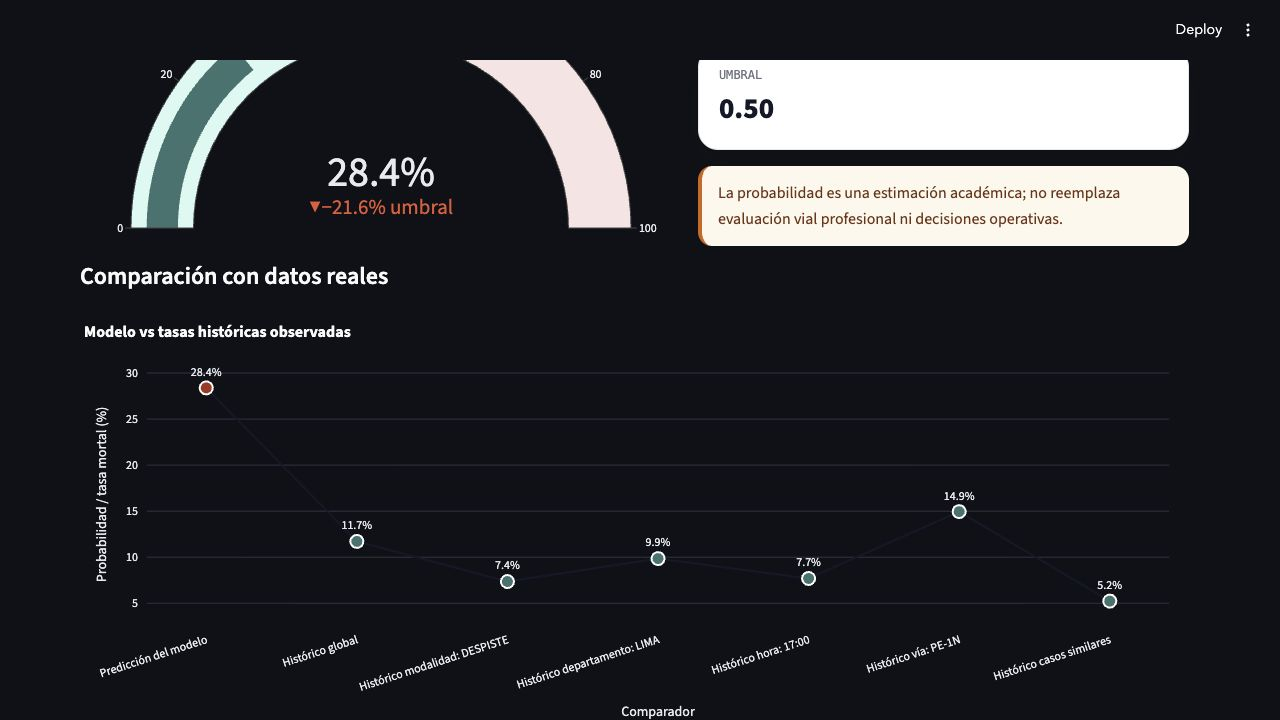
\includegraphics[width=\linewidth]{figures/gui01_prediccion.png}
    \caption{Pestaña 1: predicción de severidad con medidor \emph{gauge}.}
    \label{fig:gui01}
  \end{minipage}\hfill
  \begin{minipage}{0.49\textwidth}\centering
    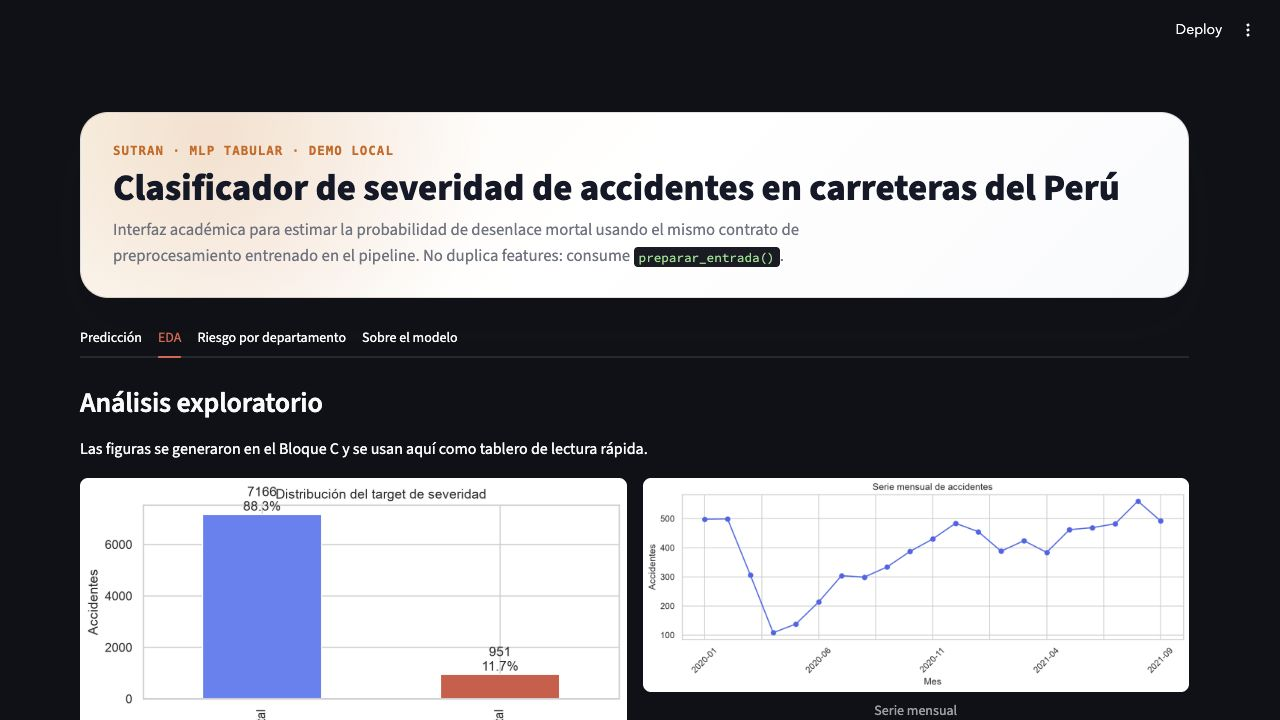
\includegraphics[width=\linewidth]{figures/gui02_eda.png}
    \caption{Pestaña 2: análisis exploratorio interactivo.}
    \label{fig:gui02}
  \end{minipage}
\end{figure}

\begin{figure}[H]
  \centering
  \begin{minipage}{0.49\textwidth}\centering
    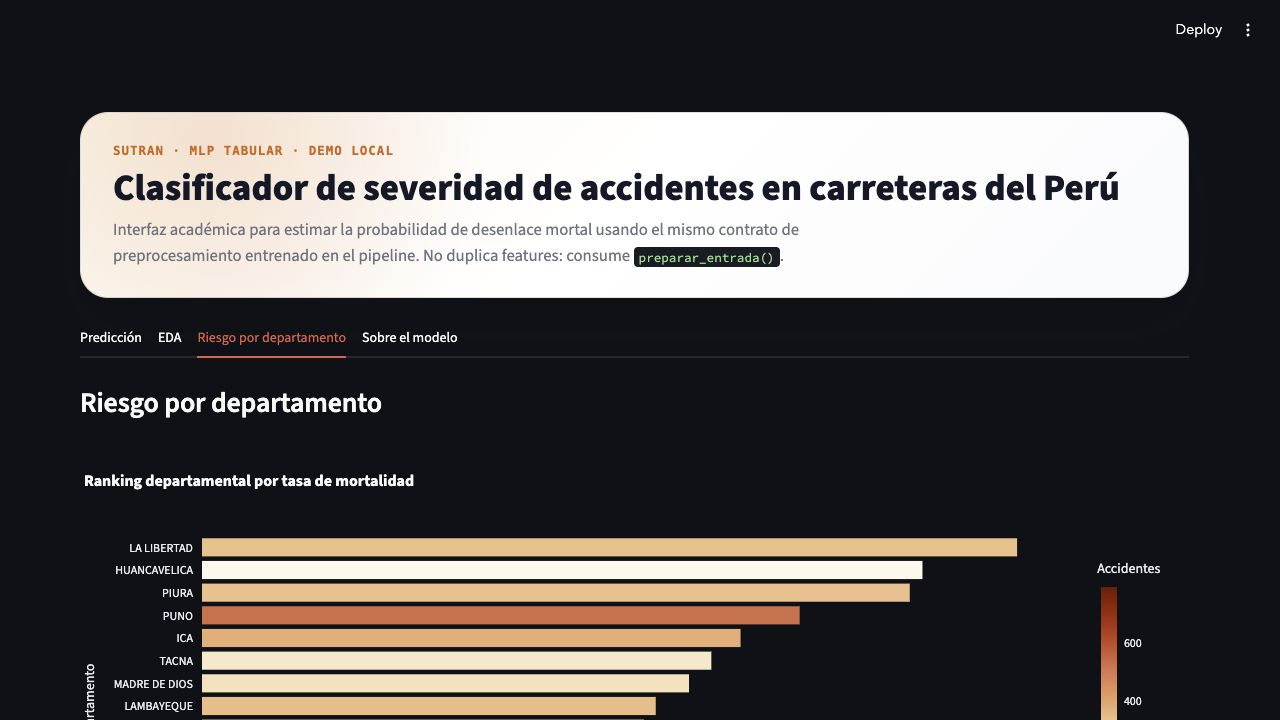
\includegraphics[width=\linewidth]{figures/gui03_riesgo_departamento.png}
    \caption{Pestaña 3: riesgo por departamento.}
    \label{fig:gui03}
  \end{minipage}\hfill
  \begin{minipage}{0.49\textwidth}\centering
    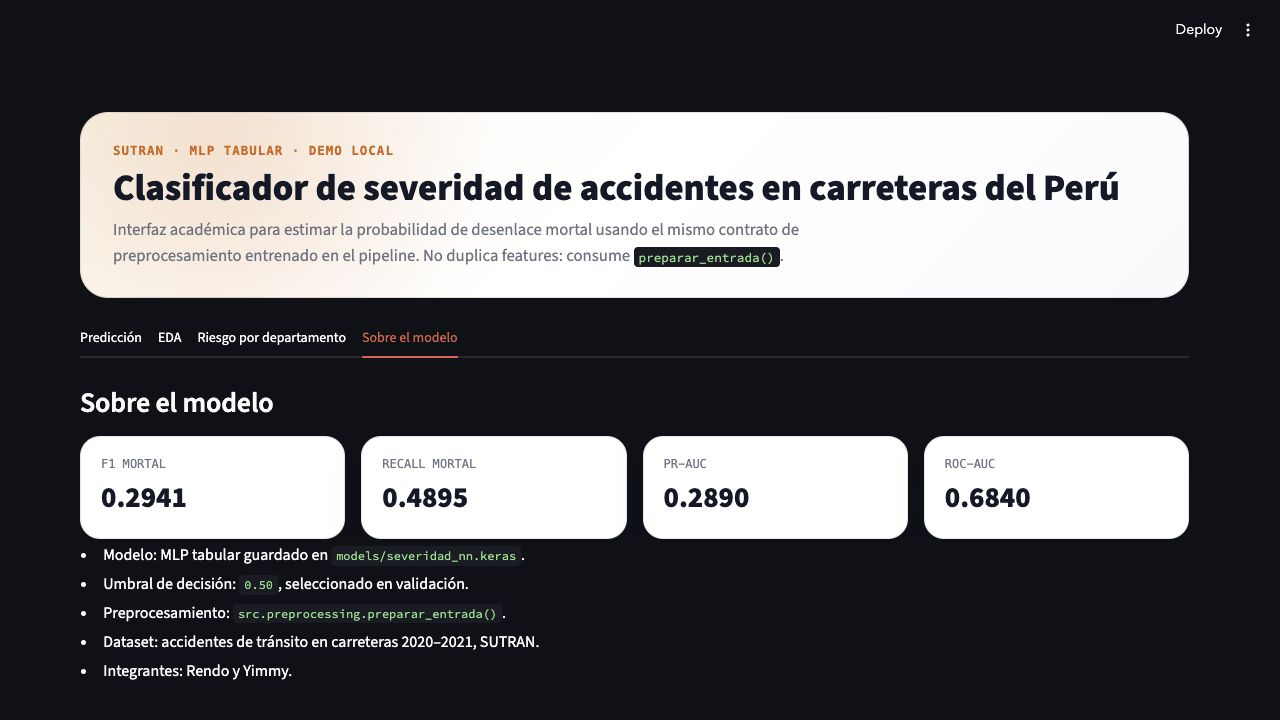
\includegraphics[width=\linewidth]{figures/gui04_sobre_modelo.png}
    \caption{Pestaña 4: sobre el modelo y comparación.}
    \label{fig:gui04}
  \end{minipage}
\end{figure}